\documentclass[10pt]{article}

\usepackage[utf8]{inputenc}
\usepackage[spanish]{babel}
\decimalpoint
\usepackage{amsmath, amssymb}
\usepackage{xcolor}
\usepackage{geometry}
\geometry{letterpaper, margin=1in}
\usepackage{graphicx}
\usepackage{hyperref}
\usepackage{float}


\title{Universidad Panamericana \\ Maestría en Ciencia de Datos \\ Econometría \\ \vspace{0.5cm} Reporte Estadístico del Estudio de Mercado de la Televisión por Cable}
\author{Enrique Ulises Báez Gómez Tagle}
\date{\today}

\begin{document}

\maketitle

\tableofcontents

\newpage

\section{Introducción}
Una empresa de televisión por cable encargó a un bufete un estudio de mercado para conocer el perfil de los clientes potenciales de una zona residencial formada por dos colonias. Las colonias constan de 12 y 25 manzanas con un total de 236 y 605 hogares, respectivamente. Mediante muestreo probabilístico (no discutido aquí) se seleccionó una muestra de ocho manzanas y cinco hogares por manzana. En cada hogar seleccionado se recabaron varias respuestas de las que presentamos solamente algunas de éstas:

\subsection{Variables del estudio}
En la Tabla~\ref{tab:variables_descripcion} se resumen las variables recolectadas en el estudio.

\begin{table}[H]
    \centering
    \caption{Descripción de las variables estudiadas}
    \label{tab:variables_descripcion}
    \begin{tabular}{llp{8cm}}
        \hline
        \# & Variable & Descripción \\ \hline
        1 & \textbf{Colonia} & Colonia a la que pertenece el hogar de la zona residencial. \\
        2 & \textbf{Manzana} & Número de manzana a la que pertenece el hogar. \\
        3 & \textbf{Adultos} & Número de adultos por hogar. \\
        4 & \textbf{Niños} & Número de niños menores de 12 años por hogar. \\
        5 & \textbf{Teles} & Número de televisores por hogar. \\
        6 & \textbf{Tipo} & Tipo de televisor que posee el hogar: blanco y negro (B), color (C), ambos (A) o ninguno (N). \\
        7 & \textbf{TVtot} & Suma del número de horas frente al televisor en la semana de todos los miembros del hogar. \\
        8 & \textbf{Renta} & Cantidad máxima de renta que el jefe del hogar estaría dispuesto a pagar por el servicio (múltiplos de \$5). \\
        9 & \textbf{Valor} & Valor catastral del hogar (miles de pesos), como aproximación al ingreso familiar. \\
        \hline
    \end{tabular}
\end{table}

\section{Respuestas a las preguntas}
En esta sección se responden las preguntas planteadas en el estudio, basándose en el análisis de los datos proporcionados.

\subsection*{A. Clasificación de variables}
Las variables se clasifican según su naturaleza en cualitativas (categóricas) o cuantitativas y, para éstas últimas, se indica si son discretas o continuas. A continuación el análisis para cada una de las variables:

\begin{itemize}
    \item \textbf{Colonia}: variable cualitativa nominal.
    \item \textbf{Manzana}: variable cualitativa nominal.
    \item \textbf{Adultos}: variable cuantitativa discreta.
    \item \textbf{Niños}: variable cuantitativa discreta.
    \item \textbf{Teles}: variable cuantitativa discreta.
    \item \textbf{Tipo}: variable cualitativa nominal.
    \item \textbf{TVtot}: variable cuantitativa continua. Aunque en este dataset tiene un salto de $1 h$ , representa la suma del tiempo de visualización y puede tomar un rango mucho más amplio.
    \item \textbf{Renta}: variable cuantitativa discreta.
    \item \textbf{Valor}: variable cuantitativa continua.
\end{itemize}

\subsection*{B. Tipo de datos}
El estudio es un \textbf{corte transversal}, pues todas las observaciones (40 hogares) fueron recolectadas en un único momento en el tiempo. No se realizaron mediciones repetidas a lo largo del tiempo, entonces no es un panel ni una serie longitudinal.

\subsection*{C. Fuente de información}
La información proviene de encuestas directas aplicadas directamente. Dado que los datos se obtuvieron específicamente para este estudio mediante un instrumento diseñado, la fuente de información es \textbf{primaria}.

\subsection*{D. Escala de medición y operaciones permitidas}
\begin{itemize}
    \item \textbf{Variables nominales} (Colonia, Manzana, Tipo): permiten conteo de frecuencias, obtención de moda y cálculo de proporciones. No se pueden sumar ni promediar.
    \item \textbf{Variables de razón} (Adultos, Niños, Teles, TVtot, Renta, Valor): todas estas variables tienen un cero absoluto y nos permiten operaciones aritméticas como suma, resta, promedios, proporciones.
\end{itemize}

\subsection*{E. Histograma del valor catastral}
La Figura~\ref{fig:hist_valor} muestra el histograma del valor catastral de los hogares (en pesos). 
Se aprecia que los valores oscilan entre aproximadamente \$80\,000 y \$370\,000. 
La frecuencia más alta se concentra en el intervalo \$120\,000–\$160\,000, con un pico secundario en \$200\,000–\$240\,000.\\
Además, la media aritmética está alrededor de \$228\,000 y la mediana en \$216\,000, lo que sugiere una ligera asimetría positiva que se observa en la cola derecha de la distribución.\\
El rango intercuartílico (de \$162\,000 a \$284\,000) muestra una dispersión moderada: el 50\% de los hogares se encuentra dentro de estos valores.\\
Existen unos cuantos valores inferiores a \$100 000 y superiores a \$350 000, lo cual indica cierta heterogeneidad en la muestra, lo cual puede servir para segmentar el mercado según la capacidad de pago.

\begin{figure}[H]   
    \centering
    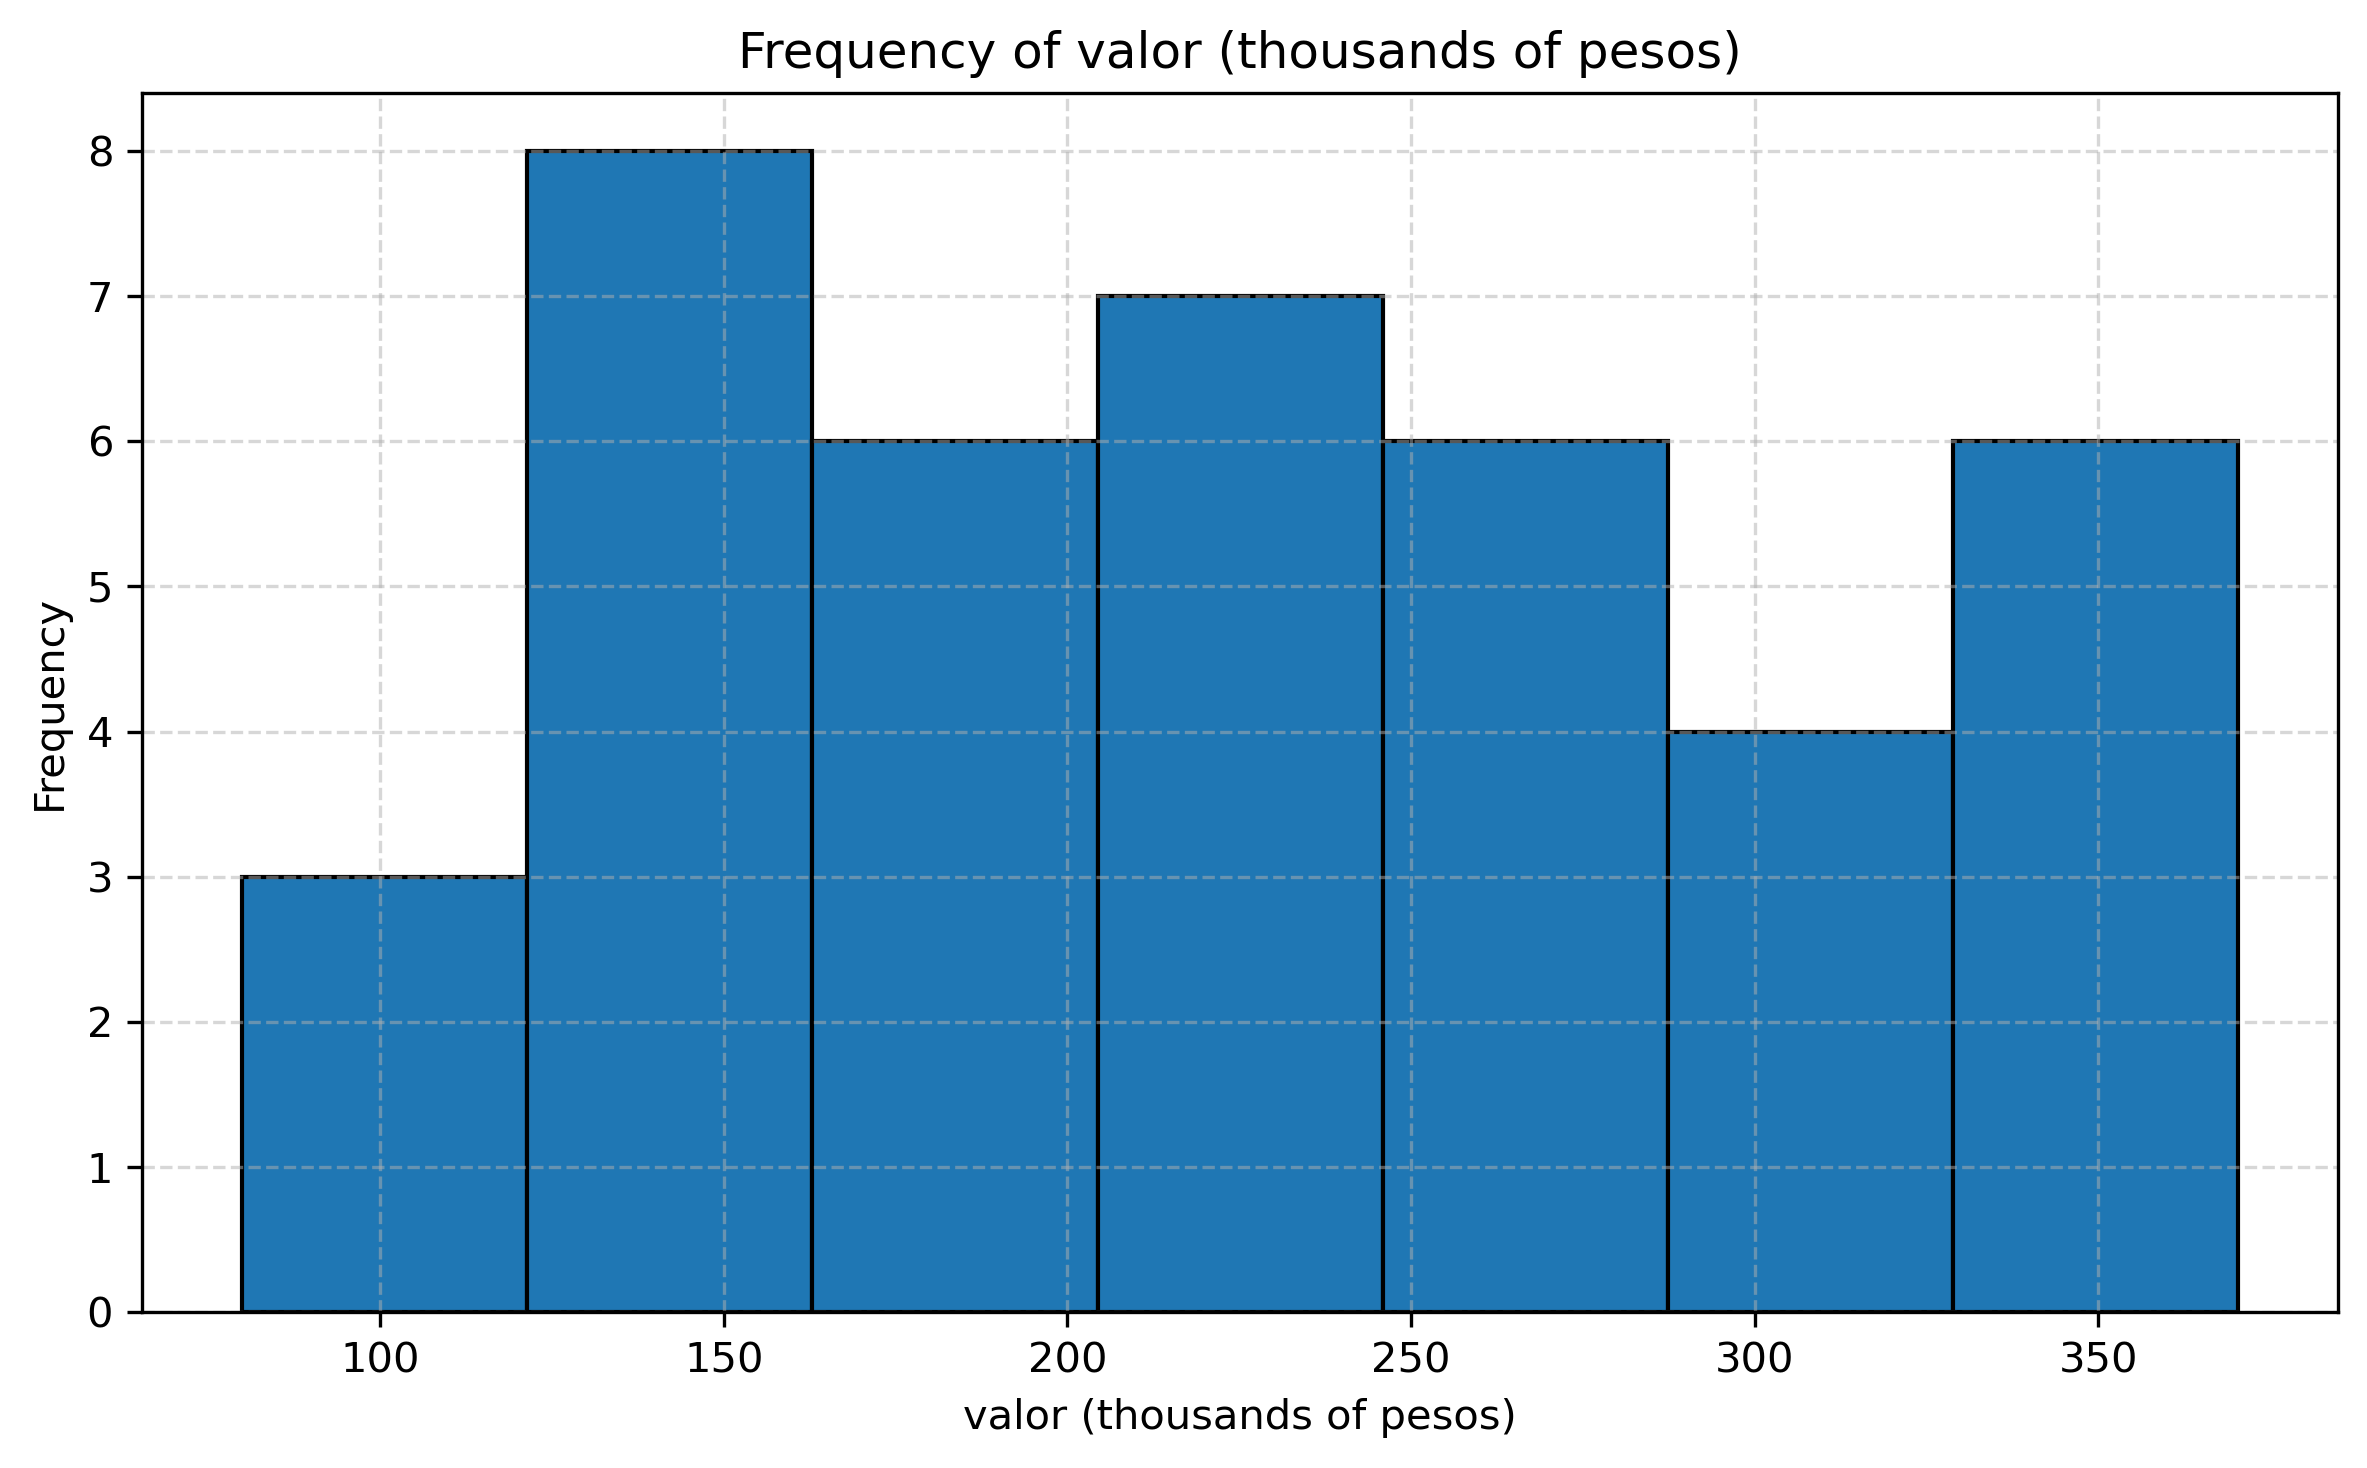
\includegraphics[width=0.75\textwidth]{../plots/python/freq_valor.png}
    \caption{Histograma del valor catastral del hogar (miles de pesos).}
    \label{fig:hist_valor}
\end{figure}

\subsection*{F. Estadísticas descriptivas}
En la Tabla~\ref{tab:stats} se presentan las principales estadísticas descriptivas de las variables cuantitativas: media ($\bar{x}$), mediana, desviación estándar (sd), mínimo y máximo. Estos valores se obtuvieron a partir de los datos proporcionados y coinciden con los resultados generados por los scripts de análisis.

\begin{table}[H]
    \centering
    \caption{Estadísticas descriptivas de las variables cuantitativas}
    \label{tab:stats}
    \begin{tabular}{lrrrrr}
        \hline
        Variable & \multicolumn{1}{c}{Media} & \multicolumn{1}{c}{Mediana} & \multicolumn{1}{c}{sd} & \multicolumn{1}{c}{Mínimo} & \multicolumn{1}{c}{Máximo} \\ \hline
        Adultos & 2.375 & 2.00 & 0.897 & 1 & 4 \\
        Niños & 1.475 & 1.50 & 1.062 & 0 & 3 \\
        Teles & 2.450 & 3.00 & 1.218 & 0 & 5 \\
        TVtot & 43.975 & 39.00 & 24.133 & 0 & 86 \\
        Renta & 58.250 & 62.50 & 17.779 & 0 & 85 \\
        Valor & 227{,}966 & 216{,}393 & 77{,}290 & 79{,}928 & 370{,}325 \\
        \hline
    \end{tabular}
\end{table}

De acuerdo con estas estadísticas, en un hogar típico de la muestra hay 2--3 adultos, 1--2 niños y 2--3 teles, dedican alrededor de 44 horas semanales a ver televisión, el jefe de hogar está dispuesto a pagar cerca de \$60 de renta y tiene una vivienda con valor catastral cercano a 228~mil pesos. La variabilidad es moderada en la mayoría de estas características, aunque las horas frente a la TV y el valor del hogar presentan una dispersión considerable.

\subsection*{G. Reporte descriptivo}
En este estudio se encuestó a un total de 40 hogares distribuidos en dos colonias; el 62.5\% de las observaciones pertenecen a la colonia~2 y el 37.5\% a la colonia~1. La población de los hogares se caracteriza por una media de 2.4 adultos y 1.5 niños, con una distribución concentrada entre 1 y 4 adultos y entre 0 y 3 niños.\\
Los hogares poseen en promedio 2.45 teles, con un máximo de cinco y algunos casos sin televisión. El tipo de TV predominante es el color (en 24 hogares), seguido de hogares con ambos tipos (10), sólo blanco y negro (4) y ninguno (2). El tiempo de exposición a la TV (\texttt{TVtot}) tiene una media de 44 horas semanales, con un rango amplio entre 0 y 86 horas, lo que indica heterogeneidad en hábitos de consumo.\\
La disposición a pagar por el servicio se acerca a \$58, con la mayoría de los hogares concentrados entre \$50 y \$70. Existe un par de hogares que no estarían dispuestos a pagar renta alguna. Finalmente, el valor catastral de las viviendas varía entre 79.9~k y 370.3~k pesos, con una media de 228~k pesos y una mediana de 216~k, sugiriendo una distribución sesgada hacia valores altos.

\section{Link al repositorio con código fuente}
\href{https://github.com/enriquegomeztagle/MCD-Econometria/tree/main/HWs/CableTVMarketStudy}{https://github.com/enriquegomeztagle/MCD-Econometria/tree/main/HWs/CableTVMarketStudy}

\end{document}
